% NOVA-Q -- GTC 2027 research poster, DRAFT v0.7 (2026-10-20). Build: pdflatex poster.tex
% Format follows the GTC 2026 poster gallery (nvidia.com/gtc/posters; 141 of the 145 poster PDFs are 43in x 24in,
% single page): centred title, authors with numbered affiliations, institution logos left and right of the title,
% framed sections with filled heading bars, References and Acknowledgments sections. No NVIDIA logos.
% Logos: National Pingtung University emblem (nptu.edu.tw emblem page), Tohoku University logo (SVG).
% Numbers: results/experiments/qaoa_cudaq_20261020 (compare.jsonl, summary.json, bench.jsonl);
% end-to-end: e2e_cfgBt_r*_20261013c rejudged.json; checker faults: results/experiments/E6_summary_dev_20261012.md.
\documentclass{article}
\usepackage[paperwidth=43in,paperheight=24in,margin=0.75in]{geometry}
\usepackage[T1]{fontenc}
\usepackage[scaled]{helvet}
\renewcommand{\familydefault}{\sfdefault}
\renewcommand{\ttdefault}{lmtt}
\usepackage{anyfontsize,graphicx,xcolor,booktabs,array,tikz,amsmath,amssymb,enumitem,sansmath}
\usepackage[poster,skins]{tcolorbox}
\usetikzlibrary{positioning,arrows.meta}
\pagestyle{empty}
\setlength{\parindent}{0pt}

% ---- type scale: body 24pt, small 19pt, heading 34pt, title 66pt (math scaled with the text)
\DeclareMathSizes{20}{20}{14}{10}
\DeclareMathSizes{16.5}{16.5}{12}{9}
\newcommand{\body}{\fontsize{20}{25}\selectfont}
\newcommand{\Small}{\fontsize{16.5}{20.5}\selectfont}
\newcommand{\Tiny}{\fontsize{14.5}{17.5}\selectfont}
\newcommand{\Head}{\fontsize{31}{36}\selectfont}
\newcommand{\Title}{\fontsize{62}{72}\selectfont}
\sansmath

\definecolor{ink}{HTML}{222222}
\definecolor{accent}{HTML}{1F4E79}
\definecolor{frame}{HTML}{9DB3C8}
\definecolor{gate}{HTML}{C2410C}
\newcommand{\gatebadge}[1]{\tikz[baseline=(g.base)]\node[circle, fill=gate, text=white, font=\bfseries\Small, inner sep=0.6mm, minimum size=6.5mm](g){#1};}
\newcommand{\key}[1]{{\bfseries #1}}
\setlist{leftmargin=1.0em, itemsep=2mm, topsep=2mm, parsep=0pt}
\setlength{\tabcolsep}{8pt}
\makeatletter\newcommand{\tabinput}[1]{\@@input #1 }\makeatother   % \input inside tabular

\begin{document}
\color{ink}\body
\begin{tcbposter}[
  poster={columns=4, rows=48, colspacing=0.45in, rowspacing=0.2in, showframe=false},
  boxes={enhanced, sharp corners, colback=white, colframe=frame, boxrule=1.2mm, left=8mm, right=8mm,
         top=6mm, bottom=6mm, fontupper=\body, valign=top,
         colbacktitle=accent, coltitle=white, fonttitle=\Head\bfseries, halign title=center,
         toptitle=3mm, bottomtitle=3mm, titlerule=0mm}]

% ================================================================ header
\posterbox[blankest, valign=center]{name=title, column=1, span=4, below=top, rowspan=7}{%
\vspace*{3mm}
\begin{minipage}[c]{0.11\linewidth}\centering
\includegraphics[height=2.7in]{logos/nptu.png}\end{minipage}\hfill
\begin{minipage}[c]{0.76\linewidth}\centering
{\Title\bfseries NOVA-Q: Verified LLM Agents From Natural Language\\[1mm]
and Open Data to QAOA on CUDA-Q\par}
\vspace{6mm}
{\fontsize{30}{36}\selectfont Chia-Chen Yang$^{1}$, \ Chia-Ho Ou$^{1,2}$\par}
\vspace{2mm}
{\fontsize{26}{32}\selectfont $^{1}$National Pingtung University, Pingtung, Taiwan \quad $^{2}$Tohoku University, Sendai, Japan
\quad cho@mail.nptu.edu.tw\par}
\end{minipage}\hfill
\begin{minipage}[c]{0.11\linewidth}\centering
\includegraphics[height=2.7in]{logos/tohoku.pdf}\end{minipage}}


% ================================================================ column 1
\posterbox[adjusted title={MOTIVATION \& CONTRIBUTIONS}]{name=intro, column=1, below=title, rowspan=15}{%
\key{Problem.} Turning a request (\emph{``place 3 EV chargers in Da'an District, Taipei, to cover the most
residents''}) into a QUBO needs data cleaning, formulation and penalty tuning expertise.

\vspace{3mm}
\key{Prior work} assumes a correct intermediate model [1], learns from user-given test cases [6], checks the
translation on standard problem types [7], or uses a hand-built model [2].

\vspace{3mm}
\key{NOVA-Q} (\textbf{N}atural-language $\to$ \textbf{O}pen-data $\to$ \textbf{V}erified \textbf{A}gents for
\textbf{Q}uantum) contributes:
\begin{enumerate}[leftmargin=1.3em, itemsep=1mm, label=\textbf{\arabic*}]
\item \key{Verify around every solve}: three gates before the solver, two after; the checker agent never sees the model.
\item \key{Cross-family checking}: a second LLM family catches 98\% of injected data faults (same family: 73\%).
\item \key{One verified QUBO, five solvers}, incl.\ QAOA on CUDA-Q.
\end{enumerate}}

\posterbox[adjusted title={WORKFLOW}]{name=pipe, column=1, below=intro, rowspan=16}{%
\centering
\resizebox{\linewidth}{!}{%
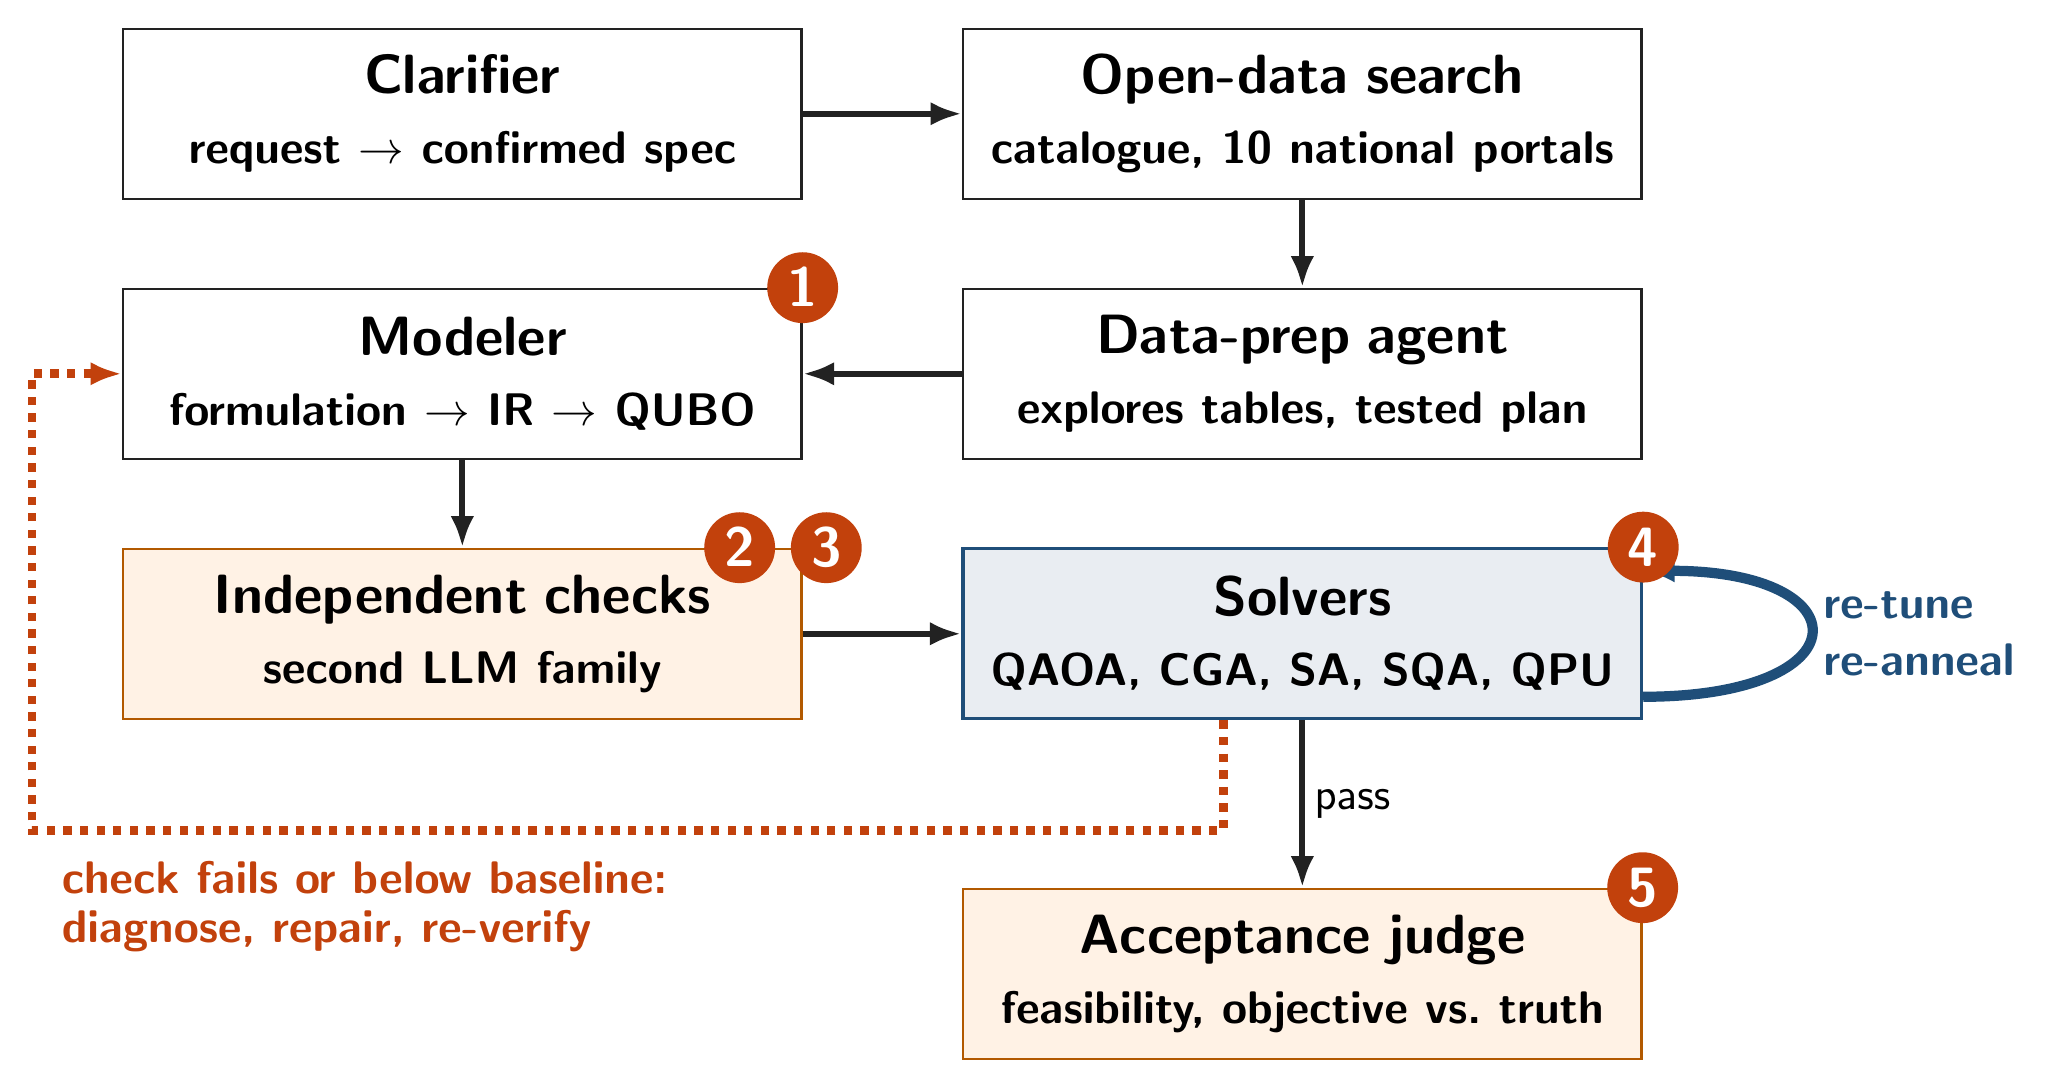
\begin{tikzpicture}[
  st/.style={draw=ink, thick, fill=white, minimum height=0.85in, text width=3.3in, align=center, font=\body},
  ck/.style={st, fill=orange!10, draw=orange!70!black},
  sv/.style={st, fill=accent!10, draw=accent, very thick},
  ar/.style={-{Latex[length=4mm]}, line width=0.8mm, draw=ink},
  gb/.style={circle, fill=gate, text=white, font=\bfseries\body, inner sep=0.8mm, minimum size=9mm}]
\node[st] (a) at (0, 0)      {\bfseries Clarifier\\\Small request $\to$ confirmed spec};
\node[st] (b) at (4.2in, 0)  {\bfseries Open-data search\\\Small catalogue, 10 national portals};
\node[st] (c) at (4.2in, -1.3in) {\bfseries Data-prep agent\\\Small explores tables, tested plan};
\node[st] (d) at (0, -1.3in) {\bfseries Modeler\\\Small formulation $\to$ IR $\to$ QUBO};
\node[ck] (e) at (0, -2.6in) {\bfseries Independent checks\\\Small second LLM family};
\node[sv] (f) at (4.2in, -2.6in) {\bfseries Solvers\\\Small QAOA, CGA, SA, SQA, QPU};
\node[ck] (g) at (4.2in, -4.3in) {\bfseries Acceptance judge\\\Small feasibility, objective vs.\ truth};
\draw[ar] (a) -- (b); \draw[ar] (b) -- (c); \draw[ar] (c) -- (d); \draw[ar] (d) -- (e);
\draw[ar] (e) -- (f); \draw[ar] (f) -- node[right, font=\Small] {pass} (g);
% inner loop on the right of the solvers
\draw[ar, draw=accent, line width=1.3mm] ([yshift=-8mm]f.east) to[out=0, in=0, looseness=4.5]
  node[right, font=\Small\bfseries, text=accent, align=left] {re-tune\\re-anneal} ([yshift=8mm]f.east);
% outer loop: from the solvers back to the modeler, around the left side
\draw[ar, draw=gate, line width=1.1mm, dashed] ([xshift=-10mm]f.south) -- ++(0,-0.55in) -| ([xshift=-0.45in]e.west)
  |- (d.west);
\node[font=\Small\bfseries, text=gate, align=left, anchor=north west, text width=3.4in]
  at ([xshift=-0.35in, yshift=-0.66in]e.south west) {check fails or below baseline:\\[-1mm]diagnose, repair, re-verify};
\node[gb] at (d.north east) {1}; \node[gb] at ([xshift=-8mm]e.north east) {2}; \node[gb] at ([xshift=3mm]e.north east) {3};
\node[gb] at (f.north east) {4}; \node[gb] at (g.north east) {5};
\end{tikzpicture}}\par
\vspace{3mm}\raggedright\Small
\gatebadge{1}--\gatebadge{5} gates. {\color{accent}\bfseries Inner loop}: solver feedback re-tunes penalties and
parameters. {\color{gate}\bfseries Outer loop}: a failed check sends the model back for repair and re-verification;
if repair fails, the verified baseline is delivered. Formulation agents from QuantumQUBO Agent [6]; the rest is new.}

\posterbox[adjusted title={REAL CITIES, OFFICIAL OPEN DATA}]{name=e2e, column=1, between=pipe and bottom}{%
\Small One sentence in, e.g.\ \emph{``Place 3 EV chargers in Da'an District to cover the most residents within 1\,km.''}
3 runs per case, independent judge.

\vspace{1.5mm}\centering
\setlength{\tabcolsep}{4pt}
\begin{tabular}{@{}l l r c@{}}
\toprule
City \& task & official source & instance (real data) & passed \\
\midrule
Taipei: EV chargers   & village census     & 53 villages, 0.28\,M people & 3/3 \\
Taipei: bike tour     & YouBike live API   & 18 stations                 & 2/3 \\
Taipei: AED zones     & AED registry       & 48 sites                    & 3/3 \\
London: ambulances    & ONS Census 2021    & 27 areas, 0.21\,M people    & 1/3 \\
Berlin: playgrounds   & Umweltatlas        & 36 sites, 0.29\,M people    & 0/3 \\
\midrule
\multicolumn{3}{@{}l}{\bfseries Passed, dev set, best of 2 LLM configs (other: 5/15)} & \bfseries 9/15 \\
\bottomrule
\end{tabular}\par}

% ================================================================ column 2
\posterbox[adjusted title={METHODOLOGY}]{name=meth, column=2, below=title, rowspan=19}{%
\key{Benchmark set.} Agent models that passed the judge, on their real data, shrunk with the pipeline's own
point-reduction tool (weighted k-means) so the optimum is known by full enumeration.

\vspace{2mm}
\begin{minipage}[c]{0.56\linewidth}\Small
\begin{tabular}{@{}l c c@{}}
\toprule
Agent-built model & points & qubits \\
\midrule
EV chargers (MCLP)        & 3--7    & 9--27 \\
Bike tour (TSP)           & 3--5    & 9--25 \\
Ambulance (p-median)      & 3--4    & 12--20 \\
AED zoning (groups)       & 3, 6, 9 & 9--27 \\
\bottomrule
\end{tabular}\\[2mm]
3 instances per size (k-means on random 80\% subsets of the real points).\\[2mm]
\textbf{Map:} 53 Da'an li (grey, size = residents), 7 representatives ($\circ$), optimal 3 chargers
({\color{accent}$\blacksquare$}) with 1\,km radius, solved exactly and by every solver.
\end{minipage}\hfill
\begin{minipage}[c]{0.42\linewidth}\centering
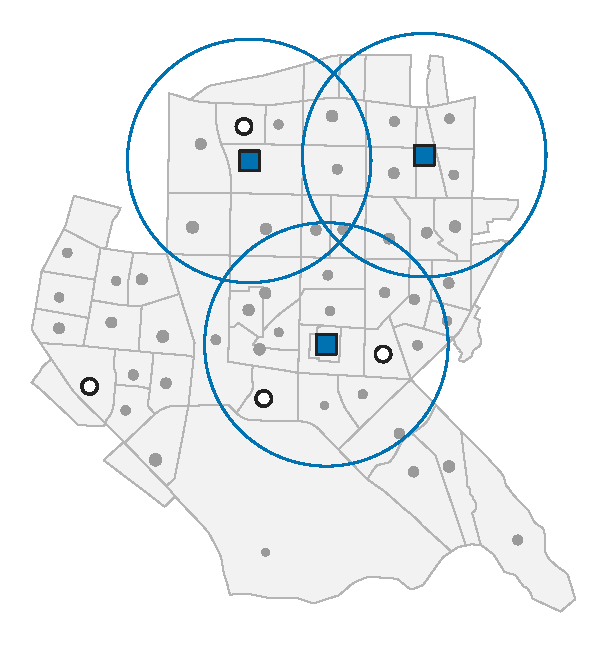
\includegraphics[width=\linewidth]{figures/map_ev_chargers_nolegend.pdf}
\end{minipage}\par
\vspace{3mm}\raggedright
\key{QAOA on CUDA-Q.} QUBO $\to$ Ising $H$,
$|\boldsymbol\gamma,\boldsymbol\beta\rangle=\prod_{l=1}^{p}e^{-i\beta_l\sum_k X_k}e^{-i\gamma_l H}|+\rangle^{\otimes n}$,
nvidia state-vector target, COBYLA, 3 restarts, $10^4$ shots.

\vspace{3mm}
\key{Other solvers.} SA, SQA (OpenJij [3]; $\beta$ tuned on 3 instances), D-Wave Advantage QPU: 1\,000 reads;
CGA: one 10\,s job. Default penalty weights for all; one run each. Samples scored on the original problem.}

\posterbox[adjusted title={VERIFICATION GATES}, colbacktitle=gate, colframe=gate!60]{name=ver, column=2, between=meth and bottom}{%
\key{Our main contribution:} gates 1--3 before solving, 4--5 after.
\begin{enumerate}[leftmargin=2.0em, itemsep=0.5mm, label=\protect\gatebadge{\arabic*}]
\item \key{Data schema \& model check}: data contract; brute force on a small instance.
\item \key{Requirement check}: a blind checker agent's mutants must be rejected.
\item \key{Data cross-check} on the raw files by a second LLM family.
\item \key{Solution check} on the original constraints and a baseline.
\item \key{Independent judge} vs.\ hand-built ground truth.
\end{enumerate}
\centering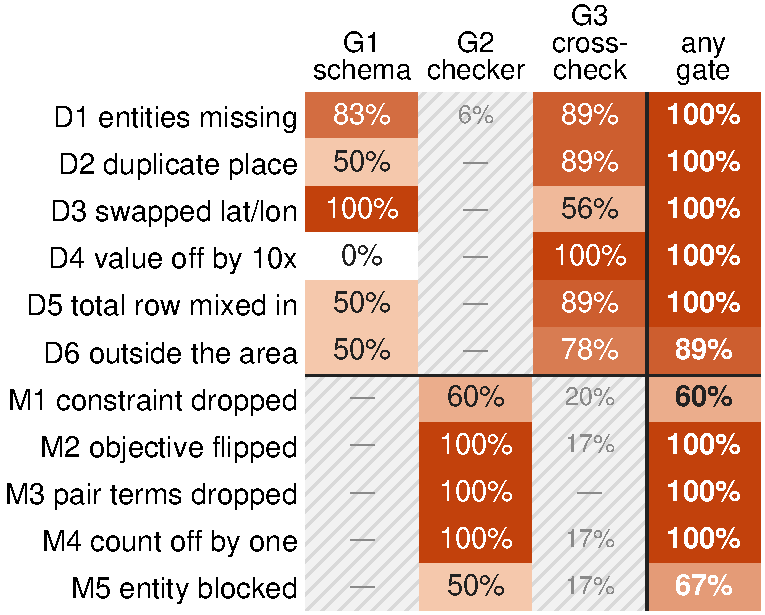
\includegraphics[height=4.5in]{figures/fault_gates.pdf}\par
\raggedright\Small Injected harmful faults, $n$=9--18 per row; doer Qwen3.6-35B-A3B, checker Gemma. Hatched = outside the
gate's scope. Caught: data 97/99, model 66/78. No false rejections in 15 verified runs (300/300 valid decisions).}

% (map example removed for space; figure: figures/map_ev_chargers.pdf)

% ================================================================ columns 3-4
\posterbox[adjusted title={RESULTS: ENERGY GAP TO THE OPTIMUM (LOWER IS BETTER)}]{name=res, column=3, span=2, below=title, rowspan=21}{%
\centering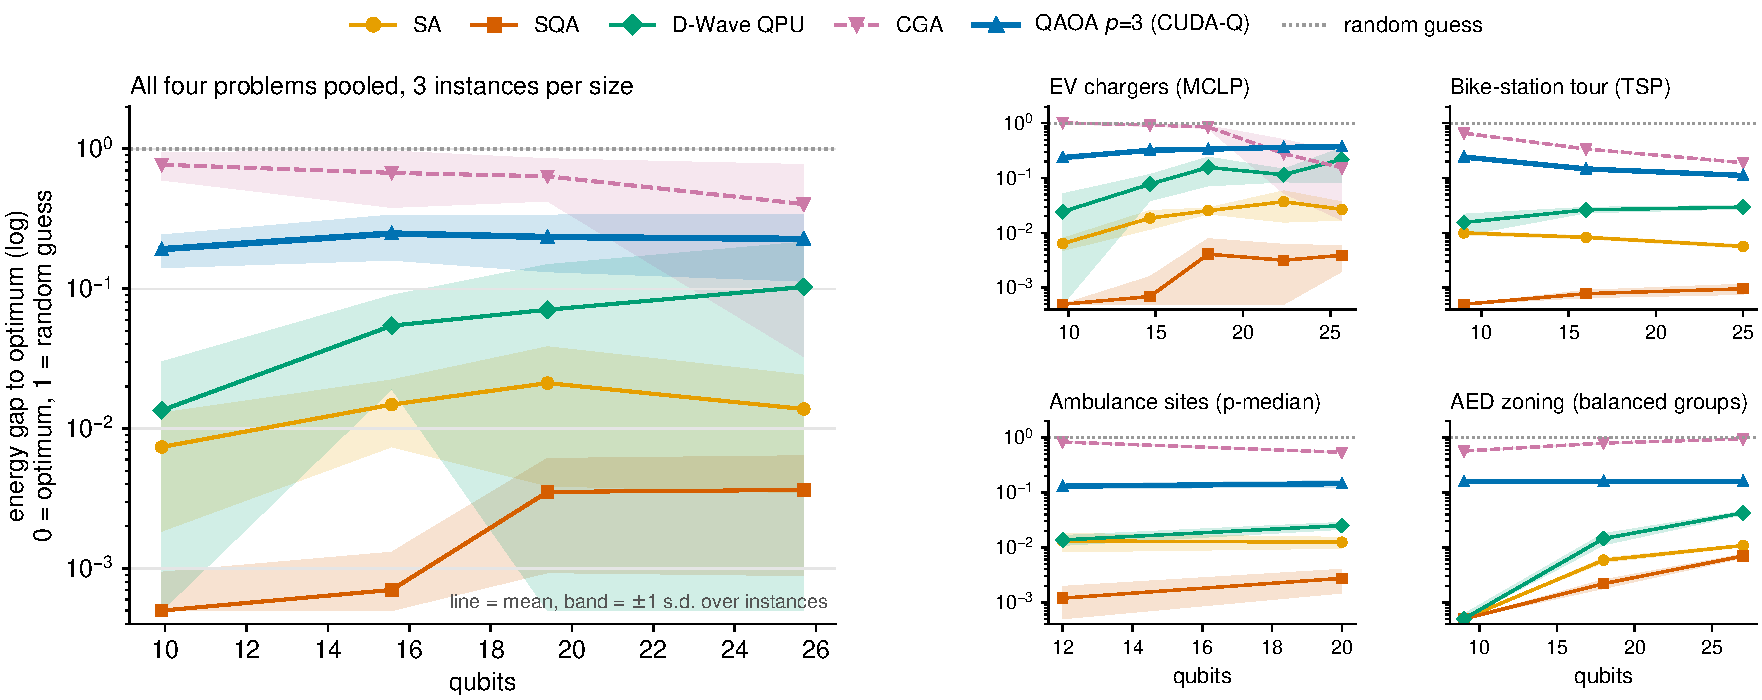
\includegraphics[width=0.96\linewidth]{figures/energy_rep.pdf}\par
\vspace{1mm}\raggedright\Small
Gap $=(E-E_{\mathrm{opt}})/(\bar E_{\mathrm{rand}}-E_{\mathrm{opt}})$, 39 instances. Median: SQA 0.001, SA 0.009, QPU 0.028,
QAOA 0.16, CGA 0.66. Optimum sampled: QAOA, SA, SQA, CGA 39/39; QPU 37/39.}

\posterbox[adjusted title={QAOA ENERGY LANDSCAPE ON 2 GPUS}]{name=tab, column=3, below=res, rowspan=12}{%
\begin{minipage}[c]{0.62\linewidth}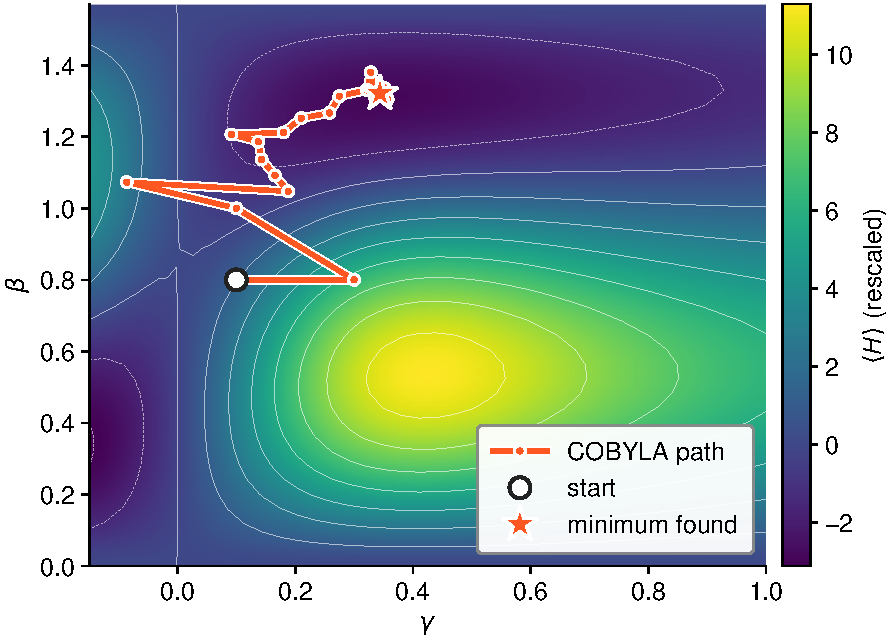
\includegraphics[width=\linewidth]{figures/qaoa_landscape.pdf}\end{minipage}\hfill
\begin{minipage}[c]{0.35\linewidth}\Small
$\langle H\rangle(\gamma,\beta)$ at $p{=}1$ (for display; results use $p{=}3$), 26-qubit EV-charger instance.\\[2mm]
\textbf{1\,600} CUDA-Q evaluations on 2$\times$ L40S (nvidia-mqpu) in \textbf{136\,s}.\\[2mm]
Orange: COBYLA path from the linear-ramp start into the low-energy valley.
\end{minipage}}

\posterbox[adjusted title={NVIDIA ACCELERATED STACK}]{name=gpu, column=4, below=res, rowspan=14}{%
\Small
\begin{itemize}
\item \key{LLM agents}: vLLM on 2$\times$ NVIDIA L40S (48\,GB), FP8 weights: Gemma-4-31B-it (Google), Qwen3.6-35B-A3B and Qwen3.6-27B (Qwen); all Apache-2.0. No cloud API.
\item \key{QAOA}: CUDA-Q 0.14, nvidia state-vector target (cuStateVec) on L40S.
\item \key{GPU annealer}: Compal CGA [2].
\end{itemize}
\vspace{2mm}\centering\Small
\begin{tabular}{l c r}
\toprule
QAOA cost evaluation ($p{=}2$, CUDA-Q 0.14) & qubits & seconds \\
\midrule
CPU (qpp-cpu)                         & 21 & 31.5 \\
GPU, 1$\times$ L40S (nvidia)          & 21 & \bfseries 0.079 \;(400$\times$) \\
GPU, 1$\times$ L40S, largest that fits         & 32 & 19.8 \\
\bottomrule
\end{tabular}\\[3mm]
\begin{tabular}{l c c c}
\toprule
nvidia-mqpu, 2$\times$ L40S & qubits & 1 GPU & 2 GPUs \\
\midrule
EV chargers (real data) & 26 & 5.5 & \bfseries 9.0 eval/s \\
Bike tour (real data)   & 25 & 4.3 & \bfseries 8.3 eval/s \\
\bottomrule
\end{tabular}\par
\vspace{2mm}\raggedright
Parallel QAOA evaluations: 1.65--1.94$\times$ throughput. nvidia-mgpu over PCIe (no NVLink) was slower:
NVLink systems (H200) are next.}

\posterbox[adjusted title={CONCLUSION \& FUTURE WORK}]{name=conc, column=3, below=tab, between=tab and bottom}{%
\Small
\begin{itemize}
\item Gates 1--3 stop wrong models before solving (98\% / 85\% of injected data / model faults).
\item One verified QUBO, five solvers. QAOA on CUDA-Q samples the optimum on every instance, but trails
the annealers: penalties cut its feasible fraction.
\item Next: constraint-preserving mixers; nvidia-mgpu on NVLink GPUs (H200).
\end{itemize}}

\posterbox[adjusted title={REFERENCES}]{name=ref, column=4, between=gpu and bottom}{%
\Tiny
[1] H.~Zhang, M.~Emu, S.~Choudhury, LLM-QUBO, AAAI-SS / arXiv:2509.00099 (2025). [2] Y.~Chou \emph{et al.}, GTC 2026 P81105. [3] OpenJij, github.com/OpenJij. [4] NVIDIA CUDA-Q 0.14. [5] E.~Farhi \emph{et al.}, QAOA, arXiv:1411.4028. [6] N.~K.~Mondal,
M.~R.~Parvez, QuantumQUBO Agent, ICML 2026 Workshop, arXiv:2609.10629. [7] K.~Sato \emph{et al.}, IEEE QCE 2025.}
\end{tcbposter}
\end{document}
